\documentclass[14pt]{extreport}
\usepackage{gost}
%\usepackage{hyperref}
%\usepackage{makecell}
\usepackage{ragged2e}
%\usepackage{graphicx}%Вставка картинок правильная
%\usepackage{float}%"Плавающие" картинки
%\usepackage{wrapfig}%Обтекание фигур (таблиц, картинок и прочего)
%\justifying

\makeatletter
\@addtoreset{figure}{part}% Reset figure numbering at every part
\makeatother
\renewcommand{\thefigure}{\arabic{figure}}% Figure number is part.figure
\renewcommand{\thetable}{\arabic{table}}

%Тут можно вставить дополнительные пакеты

\begin{document}
    \pagestyle{empty} %  выключаем нумерацию
    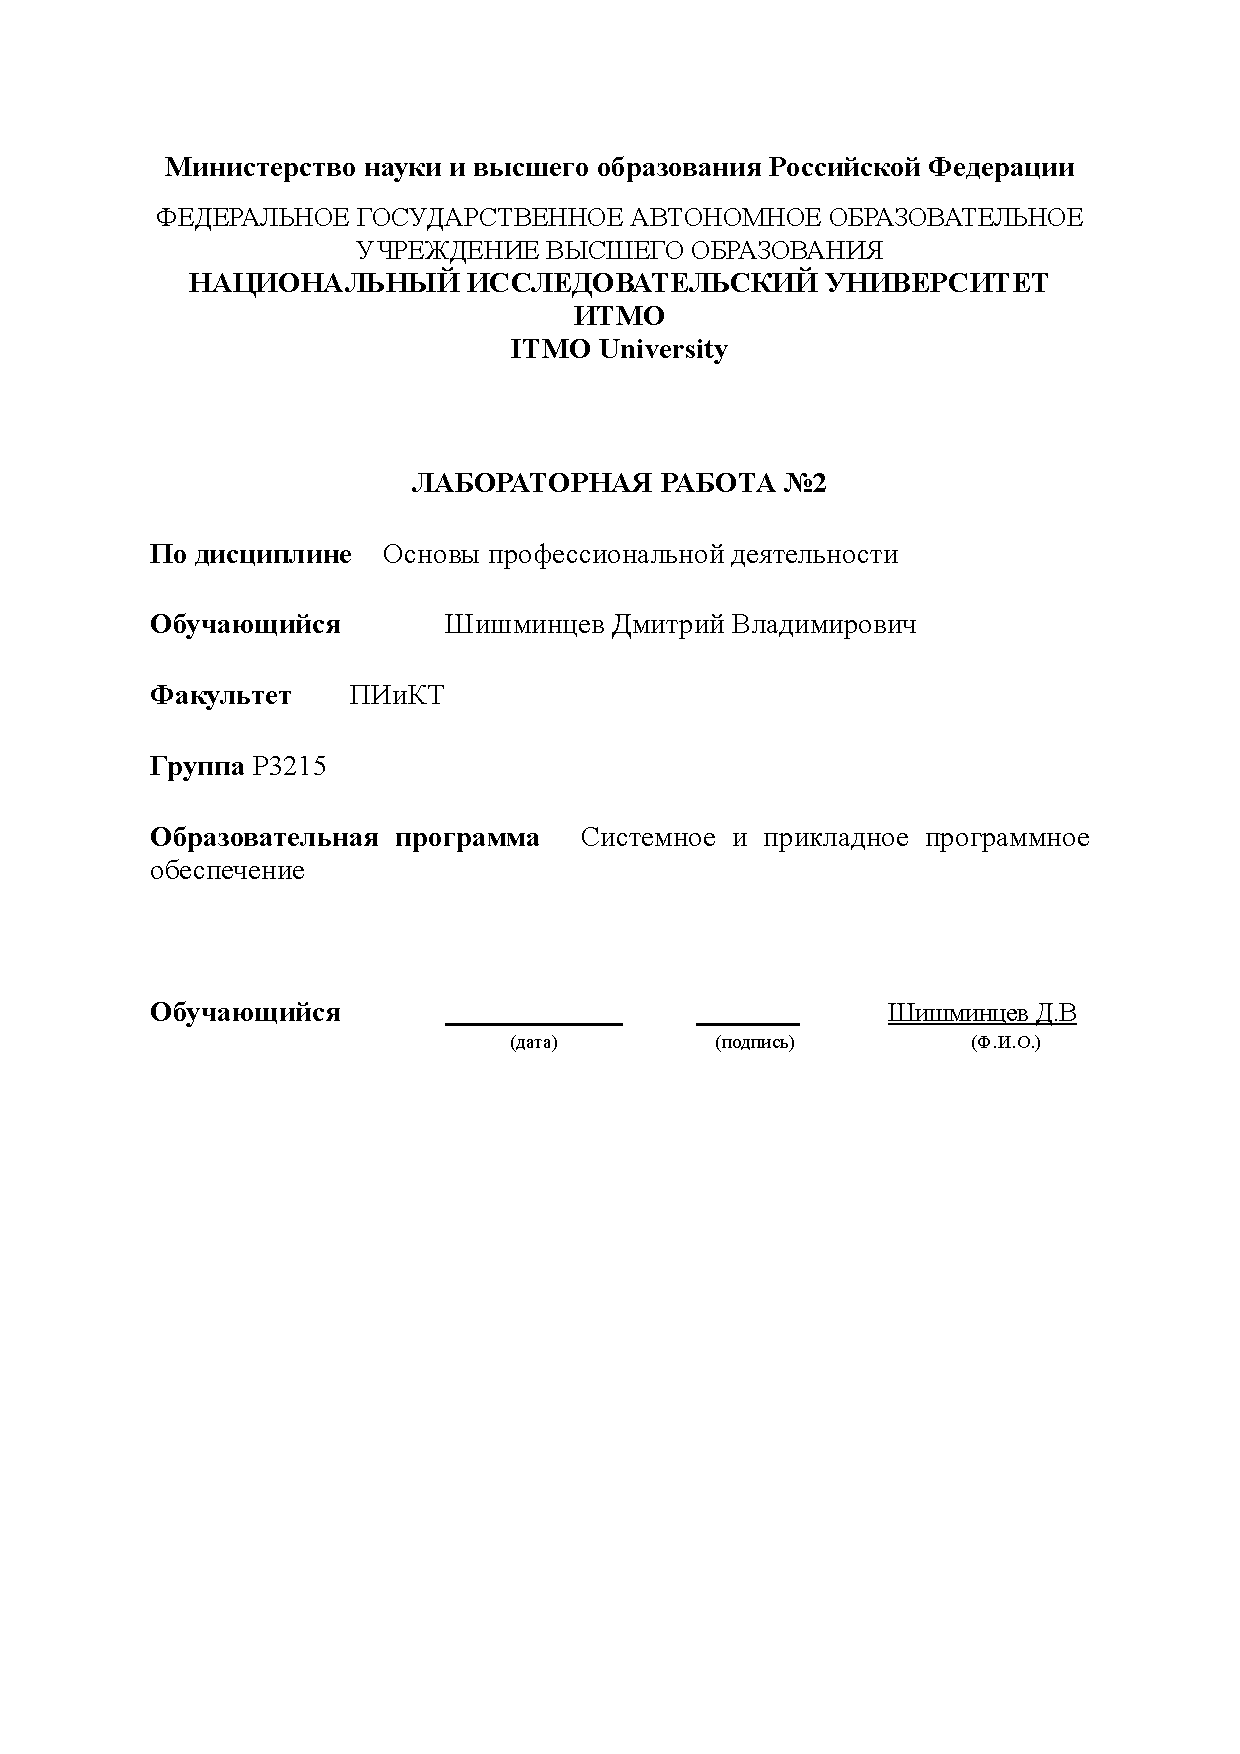
\includepdf[pages=-,pagecommand={}]{title_page.pdf}

    \pagestyle{plain} % включаем нумерацию
    \tableofcontents
    \intro Задание по базовой электронной вычислительной машине (ЭВМ) предполагает анализ программы, определение её функции, области представления и области допустимых значений исходных данных и результатов. В процессе выполнения задания требуется также провести трассировку программы и предложить вариант с уменьшенным числом команд. Этот анализ поможет понять, как программа взаимодействует с данными и как можно оптимизировать её выполнение.

    \chapter{Текст задания}
        По выданному преподавателем варианту восстановить текст заданного варианта программы и подпрограммы (программного комплекса), определить предназначение и составить его описание, определить область представления и область допустимых значений исходных данных и результата, выполнить трассировку программного комплекса.

        \begin{figure}[!h]
            \centering
            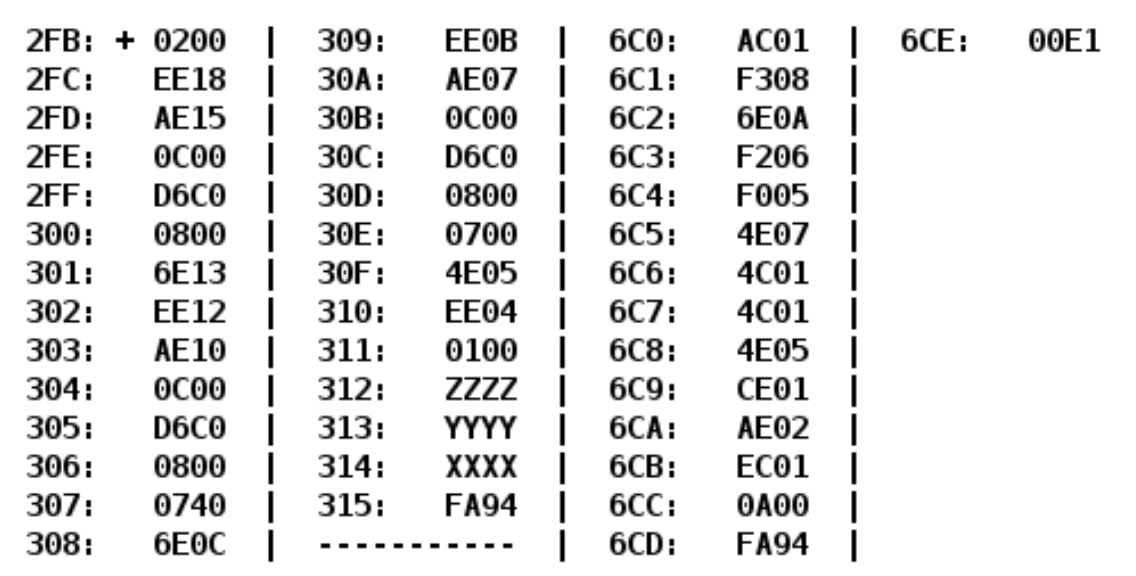
\includegraphics[width=0.8\linewidth]{task.png}
            \caption{Картинка задания}

        \end{figure}


    \chapter{Таблица исходной программы}
        \begin{table}[h]

            \centering
            \begin{tabular}{|c|c|c|c|}
                \hline
                Адрес & Команда & Мнемоника & Комментарий \\ \hline \hline
                2FB & 0200 & CLA        & AC = 0\\ \hline
                2FC & EE18 & ST IP+24   & C [315] = 0\\ \hline
                2FD & AE15 & LD IP+21   & AC = X [313]\\ \hline
                2FE & 0C00 & PUSH       & AC => STACK \\ \hline
                2FF & D6C0 & CALL 6C0   & Вызов процедуры\\ \hline
                300 & 0800 & POP        & STACK => AC\\ \hline
                301 & 6E13 & SUB IP+19  & AC = AC - C [315]\\ \hline
                302 & EE12 & ST IP+18   & C = AC \\ \hline
                303 & AE10 & LD IP+16   & AC = Y \\ \hline
                304 & 0C00 & PUSH       & AC => STACK\\ \hline
                305 & D6C0 & CALL 6C0   & Вызов процедуры\\ \hline
                306 & 0800 & POP        & STACK => AC\\ \hline
                307 & 0740 & DEC        & AC--\\ \hline
                308 & 630C & SUB IP+12  & AC=AC-C\\ \hline
                309 & EE0B & ST IP+11   & C = AC\\ \hline
                30A & AE07 & LD IP+7    & AC = Z\\ \hline
                30B & 0C00 & PUSH       & AC => STACK\\ \hline
                30C & D6C0 & CALL 6C0   & Вызов процедуры\\ \hline
                30D & 0800 & POP        & STACK=>AC\\ \hline
                30E & 0700 & INC        & AC++\\ \hline
                30F & 4E05 & ADD IP+5   & AC = AC + C\\ \hline
                310 & EE04 & ST IP+4    & C = AC\\ \hline
                311 & 0100 & HLT        & STOP\\ \hline \hline
                312 & ???? &            & Z \\ \hline
                313 & ???? &            & Y \\ \hline
                314 & ???? &            & X \\ \hline
                315 & FA94 &            & C \\ \hline
            \end{tabular}\label{tab:table}
        \end{table}

    \chapter{Таблица подпрограммы}
        \begin{table}[h]

            \centering
            \begin{tabular}{|c|c|c|c|}
                \hline
                Адрес & Команда & Мнемоника & Комментарий \\ \hline
                6C0 & AC01 & LD SP+1    & STACK=>AC\\ \hline \hline
                6C1 & F308 & BPL 08     & IF N==0 => JUMP 6C9\\ \hline
                6C2 & 6E0A & SUB IP+10  & AC = AC - C2 [6CE]\\ \hline
                6C3 & F206 & BMI 06     & IF N == 1 => JUMP 6C9\\ \hline
                6C4 & F005 & BEQ 05     & IF Z == 1 => JUMP 6C9\\ \hline
                6C5 & 4E07 & ADD IP+7   & AC = AC + C1\\ \hline
                6C6 & 4C01 & ADD SP+1   & AC = AC + X\\ \hline
                6C7 & 4C01 & ADD SP+1   & AC = AC + X\\ \hline
                6C8 & 4E05 & ADD IP+5   & AC = AC + C2\\ \hline
                6C9 & CE01 & JUMP IP+1  & Переход к 6CB\\ \hline
                6CA & AE02 & LD IP+2    & AC = AC + C1 [6CD]\\ \hline
                6CB & EC01 & ST SP+1    & AC => STACK \\ \hline
                6CC & 0A00 & RET        & \\ \hline \hline
                6CD & FA94 &            & C1 \\ \hline
                6CE & 00E1 &            & C2 \\ \hline
            \end{tabular}\label{tab:table}
        \end{table}

    \chapter{Анализ исходной программы}

    2FB - 311 - Программа

    312 - Переменная Z

    313 - Переменная Y

    314 - Переменная X

    315 - Результат

    6C0 - 6CC - Подпрограмма

    6CD - Константа для подпрограмммы

    6CE - Константа для подпрограммы
    \section{Реализуемая функция}
            $R = f(z) + f(x) - f(y) $ \\


        $f(x) =$\begin{cases}
                        -1388, x >= 0 \\
                        -1388, -2^{15} + 1388 < x <= 0 \\
                        3X + 225, -2^{15} <= x <= 2^{15} - 1388
            \end{cases}

    \section{Область допустимых значений}

        Область значений результата: [64148]

        Область допустимых значений:
\\

            \begin{cases}
                -2^{15} < x <-2^{15} + 225 \\
                -2^{15} < y <-2^{15} + 225 \\
                0< z <2^{15} - 1 \\
            \end{cases}

            \begin{cases}
                -2^{15} < x <-2^{15} + 225 \\
                0< y <2^{15} - 1 \\
                -2^{15} < z <-2^{15} + 225 \\
            \end{cases}

            \begin{cases}
                0< x <2^{15} - 1 \\
                -2^{15} < y <-2^{15} + 225 \\
                -2^{15} < z <-2^{15} + 225 \\
            \end{cases}
        \begin{landscape}
            \chapter{Трассировка программы}
            \begin{table}[!h]
                \centering
                \begin{tabular}{|l|l|l|l|l|l|l|l|l|l|l|l|l|}
                    \hline
                    Адр & Знчн & IP & CR & AR & DR & SP & BR & AC & PS & NZVC & Адр & Знчн \\
                    \hline
                    2FB & 0200 & 2FB & 0000 & 000 & 0000 & 000 & 0000 & 0000 & 004 & 0100&& \\
                    2FB & 0200 & 2FC & 0200 & 2FB & 0200 & 000 & 02FB & 0000 & 004 & 0100 &&\\
                    2FC & EE18 & 2FD & EE18 & 315 & 0000 & 000 & 0018 & 0000 & 004 & 0100 & 315 & 0000 \\
                    2FD & AE15 & 2FE & AE15 & 313 & 0000 & 000 & 0015 & 0000 & 004 & 0100&& \\
                    2FE & 0C00 & 2FF & 0C00 & 7FF & 0000 & 7FF & 02FE & 0000 & 004 & 0100 & 7FF & 0000 \\
                    2FF & D6C0 & 6C0 & D6C0 & 7FE & 0300 & 7FE & D6C0 & 0000 & 004 & 0100 & 7FE & 0300 \\
                    6C0 & AC01 & 6C1 & AC01 & 7FF & 0000 & 7FE & 0001 & 0000 & 004 & 0100&& \\
                    6C1 & F308 & 6CA & F308 & 6C1 & F308 & 7FE & 0008 & 0000 & 004 & 0100&& \\
                    6CA & AE02 & 6CB & AE02 & 6CD & FA94 & 7FE & 0002 & FA94 & 008 & 1000 &&\\
                    6CB & EC01 & 6CC & EC01 & 7FF & FA94 & 7FE & 0001 & FA94 & 008 & 1000 & 7FF & FA94 \\
                    6CC & 0A00 & 300 & 0A00 & 7FE & 0300 & 7FF & 06CC & FA94 & 008 & 1000&& \\
                    300 & 0800 & 301 & 0800 & 7FF & FA94 & 000 & 0300 & FA94 & 008 & 1000&& \\
                    301 & 6E13 & 302 & 6E13 & 315 & 0000 & 000 & 0013 & FA94 & 009 & 1001&& \\
                    302 & EE12 & 303 & EE12 & 315 & FA94 & 000 & 0012 & FA94 & 009 & 1001 & 315 & FA94 \\
                    303 & AE10 & 304 & AE10 & 314 & FF00 & 000 & 0010 & FF00 & 009 & 1001 &&\\
                    304 & 0C00 & 305 & 0C00 & 7FF & FF00 & 7FF & 0304 & FF00 & 009 & 1001 & 7FF & FF00 \\
                    305 & D6C0 & 6C0 & D6C0 & 7FE & 0306 & 7FE & D6C0 & FF00 & 009 & 1001 & 7FE & 0306 \\
                    6C0 & AC01 & 6C1 & AC01 & 7FF & FF00 & 7FE & 0001 & FF00 & 009 & 1001 &&\\
                    6C1 & F308 & 6C2 & F308 & 6C1 & F308 & 7FE & 06C1 & FF00 & 009 & 1001 &&\\
                    6C2 & 6E0A & 6C3 & 6E0A & 6CD & FA94 & 7FE & 000A & 046C & 001 & 0001 &&\\
                    6C3 & F206 & 6C4 & F206 & 6C3 & F206 & 7FE & 06C3 & 046C & 001 & 0001 &&\\
                    6C4 & F005 & 6C5 & F005 & 6C4 & F005 & 7FE & 06C4 & 046C & 001 & 0001 &&\\
                    \hline
                \end{tabular}

            \end{table}
            \begin{table}[h]
                \centering
                \begin{tabular}{|l|l|l|l|l|l|l|l|l|l|l|l|l|}
                    \hline
                    6C5 & 4E07 & 6C6 & 4E07 & 6CD & FA94 & 7FE & 0007 & FF00 & 008 & 1000 &&\\
                    6C6 & 4C01 & 6C7 & 4C01 & 7FF & FF00 & 7FE & 0001 & FFFE & 009 & 1001 &&\\
                    6C7 & 4C01 & 6C8 & 4C01 & 7FF & FF00 & 7FE & 0001 & FFFD & 009 & 1001 &&\\
                    6C8 & 4E05 & 6C9 & 4E05 & 6CE & 00E1 & 7FE & 0005 & FDE1 & 008 & 1000 &&\\
                    6C9 & CE01 & 6CB & CE01 & 6C9 & 06CB & 7FE & 0001 & FDE1 & 008 & 1000 &&\\
                    6CB & EC01 & 6CC & EC01 & 7FF & FDE1 & 7FE & 0001 & FDE1 & 008 & 1000 & 7FF & FDE1 \\
                    6CC & 0A00 & 30D & 0A00 & 7FE & 030D & 7FF & 06CC & FDE1 & 008 & 1000 && \\
                    30D & 0800 & 30E & 0800 & 7FF & FDE1 & 000 & 030D & FDE1 & 008 & 1000 &&\\
                    30E & 0700 & 30F & 0700 & 30E & 0700 & 000 & 030E & FDE0 & 009 & 1001 &&\\
                    30F & 4E05 & 310 & 4E05 & 315 & 034C & 000 & 0005 & 042B & 000 & 0000 &&\\
                    310 & EE04 & 311 & EE04 & 315 & 042B & 000 & 0004 & 042B & 000 & 0000 & 315 & 042B \\
                    311 & 0100 & 312 & 0100 & 311 & 0100 & 000 & 0311 & 042B & 000 & 0000 &&\\
                    \hline
                \end{tabular}
                \end{table}
        \end{landscape}


    \conclusions Исследование программы на базовой ЭВМ позволяет глубже понять её работу и оптимизировать выполнение, что важно для повышения эффективности и экономии ресурсов. Анализ функции, области представления и области допустимых значений данных, трассировка программы и оптимизация команд помогут более эффективно использовать ресурсы ЭВМ и достичь более эффективных результатов в вычислениях.

\end{document}